%\documentclass[11pt]{amsart}
\documentclass[12pt]{article}
\usepackage[top=0.6in,bottom=.5in,left=.8in,right=.8in]{geometry}
\usepackage{geometry}                % See geometry.pdf to learn the layout options. There are lots.
\geometry{letterpaper}                   % ... or a4paper or a5paper or ... 
%\geometry{landscape}                % Activate for for rotated page geometry
%\usepackage[parfill]{parskip}    % Activate to begin paragraphs with an empty line rather than an indent
\usepackage{graphicx}
\usepackage{amsmath}
\usepackage{amssymb}
\usepackage{epstopdf}
\usepackage{tikz}
\usetikzlibrary{arrows}
\usepackage{algpseudocode}
\DeclareGraphicsRule{.tif}{png}{.png}{`convert #1 `dirname #1`/`basename #1 .tif`.png}
\linespread{1.5}

\title{Hardware RSA Accelerator}
\author{Group 3: Ariel Anders, Timur Balbekov, Neil Forrester}
%\date{}                                           % Activate to display a given date or no date

\begin{document}

\maketitle

\section{Overview}
Our project is implementing the RSA cryptographic algorithm in Bluespec.
The benefits of doing this in hardware are higher performance, reduced power usage and size, and cost.
Having reusable IP that implements RSA would allow a device manufacturer to skip the inclusion
of a processor in a device that requires secure communications, but otherwise wouldn't need one. 

An example application of our preliminary proposal could be an intelligence agencies' covert listening device
with the added ability of secure communication through RSA protocol.
Specialized hardware is useful here because the device needs to be small,
without excessive power consumption, and the ability to run for long periods of time. 

Alternatively, suppose you were designing a high performance router to create a secure VPN between remote sites,
so that it appears that all the computers at all sites are on the local network.
Keeping latency as low as possible, and throughput as high as possible, would be vital.
Hardware support for Public Key Cryptography, such as RSA,
could play an essential component in developing this router.

The main challenges we foresee in implementing RSA in Bluespec are creating a multi-precision arithmetic library
with support for modulo, exponentiation, and multiplication.
Once those problems are solved, the only remaining issue is writing a sensible interface.

\section{Algorithms}
All of our high-level RSA modules will be built around a single module that does modular exponentiation.
Unless some unforeseen detail necessitates a change, this module will employ the Right-to-left binary algorithm
(which we believe will be a good compromise between speed, memory usage, and complexity).
The goal of the algorithm is to calculate $b^e \bmod m$ for very large values of $b$, $e$, and $m$.
If the bits of $e$ are $e_1, e_2 \dots e_n$:
\begin{equation}
e = \sum_{i = 0}^{n} e_i 2^i
\end{equation}
then:
\begin{equation}
b^e = \prod_{i = 0}^{n} e_i b^{(2^i)}
\end{equation}
and since:
\begin{equation}
a * b \bmod m = (a \bmod m) * (b \bmod m) \bmod m
\end{equation}
then every intermediate result can be taken modulo $m$ to keep the size of intermediate results manageable.
Therefore, the following algorithm will compute $b^e \bmod m$ in a reasonable amount of time and memory:
\begin{algorithmic}
\State $b$, $e$, and $m$ are the inputs to the algorithm.
\State $c \gets 1$
\While{$e > 0$}
	\If{$e \bmod 2 = 1$}
		\State $c \gets c * b \bmod m$
	\EndIf
	\State $b \gets b * b \bmod m$
	\State $e \gets \lfloor e / 2 \rfloor$
\EndWhile
\State $c$ is the result of the algorithm.
\end{algorithmic}
This very naturally suggests a circular pipeline in hardware.
If parallelism is desired, then multiple circular pipelines may be put in parallel,
with some logic at the front and back to manage handing out jobs to different circular pipelines,
and collecting the results.

The only remaining problem is performing multiplication, modulo, and bit shifting
on integers that are thousands of bits long.
If it had turned out to be practical to simply instantiate registers of types like {\tt Int\#(1024)},
and perform combinational operations on them by writing {\tt a~*~b}, {\tt a~\%~m}, and {\tt a~>>~1},
then that would have been fantastic.
However, it appears that this is not the case.
The timing violations require us to handle large integers in smaller chunks.

Upon further reflection however, we believe that a compromise approach will be most practical.
Our current plan is to instantiate registers of types like {\tt Int\#(1024)}, and operate on those.
This will make combinational multiplies and divides impossible.
However, if we use the interleaved modular multiplication algorithm,
neither of these will be necessary, as it requires only bit shifts, additions, and comparisons,
which shouldn't take up excessive area.
If additions produce long combinational delays,
we could write an addition module that operates on chunks of the number at a time,
and does something like a pipelined carry-lookahead adder.
Hopefully this won't be necessary though.

Here is the algorithm for Interleaved modular multiplication.
$N$ is the size of the numbers, in bits. For example, $N = 1024$.
Also, $x_i$ is the $i$th bit of $x$.
\begin{algorithmic}
\State $x$, $y$, and $m$ are the inputs to the algorithm.
\State $p \gets 0$
\State $i \gets N - 1$
\While{$i \geq 0$}
	\State $p \gets p * 2$
	\If{$x_i = 1$}
		\State $p \gets p + y$
	\EndIf
	\If{$p \geq m$}
		\State $p \gets p - m$
	\EndIf
	\If{$p \geq m$}
		\State $p \gets p - m$
	\EndIf
  \State $i \gets i - 1$
\EndWhile
\State $p$ is the result of the algorithm.
\end{algorithmic}

\section{Implementation in C}
We have a working implementation of all our algorithms in C, that we wrote from scratch.
Performance is terrible in comparison to libgcrypt,
but libgcrypt was written by more experienced people who had more time to spend on it,
so we think this is acceptable.
C, of course, is unable to operate directly on 1024 bit integers,
so we store them as arrays of 16 bit unsigned integers.
As a result, performing bit shifts, additions, and comparisons
takes somewhat more code than it would take to perform the corresponding operations in Bluespec.
However, since we have now written a C implementation that does all the operations on chunked integers,
we now feel confident in our ability to pipeline or otherwise break up
any operations we find to be too big or long in our Bluespec implementation.

\section{Microarchitecture}
Our project is divided into two important modules.
One module performs modular exponentiaton,
while the other performs modular multiplication.
The modular exponentiator instantiates two modular multipliers.
The high level diagram in Figure \ref{fig-top} depicts the interface between
the modular multipliers and the modular exponentiator
(though only one multiplier is shown for simplicity).

The current plan is that large integers of (for example) 1024 bits
will be represented in Bluespec as {\tt Int\#(1024)}.
This will probably be practical, as we never instantiate combinational multipliers on these types,
only bit shifts, adders, and comparators, which shouldn't take up much area. However, performing
comparisons and arithmetic on long bit lengths will adversely affect the cycle time of the design.
In performance critical modules, like the modular multiplier, it will be highly beneficial
to operate on the string in chunks: for example, the 64 hardware DSP48 blocks can synthesize
a long add/subtract chain using internal routing resources. 

\begin{figure}
  \begin{centering}
    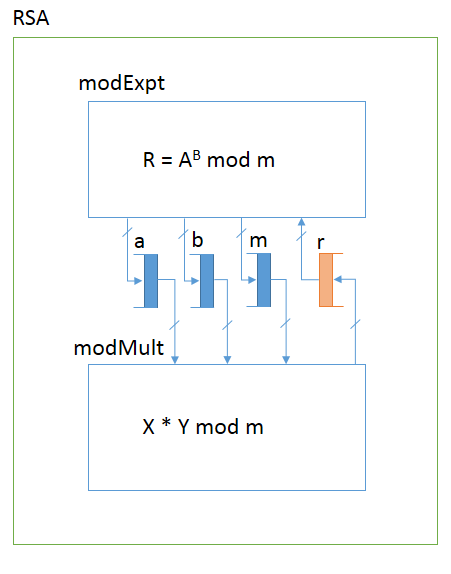
\includegraphics[scale=1]{top_level.png}
    \caption{High level overview. Note that only one of two multipliers is depicted.}
    \label{fig-top}
  \end{centering}
\end{figure}

\subsection{Right to Left Binary Modular Exponentiator}
The modular exponentiator is a circular pipeline (depicted in Figure \ref{fig-expt}).
On each cycle of the pipeline it supplies inputs to the two multipliers.
When the multipliers complete, it stores the results back into the registers.
However one result is discarded if the low bit of {\tt e} is 0.
In fact, our actual implementation will probably not invoke the multiplier
if its result will be discarded anyway.
However, this is simply an optimization, and doesn't hugely affect the overall plan.
On every iteration, the value of {\tt e} is right-shifted by one bit.
When {\tt e} is zero, the loop terminates.

\begin{figure}
  \begin{centering}
    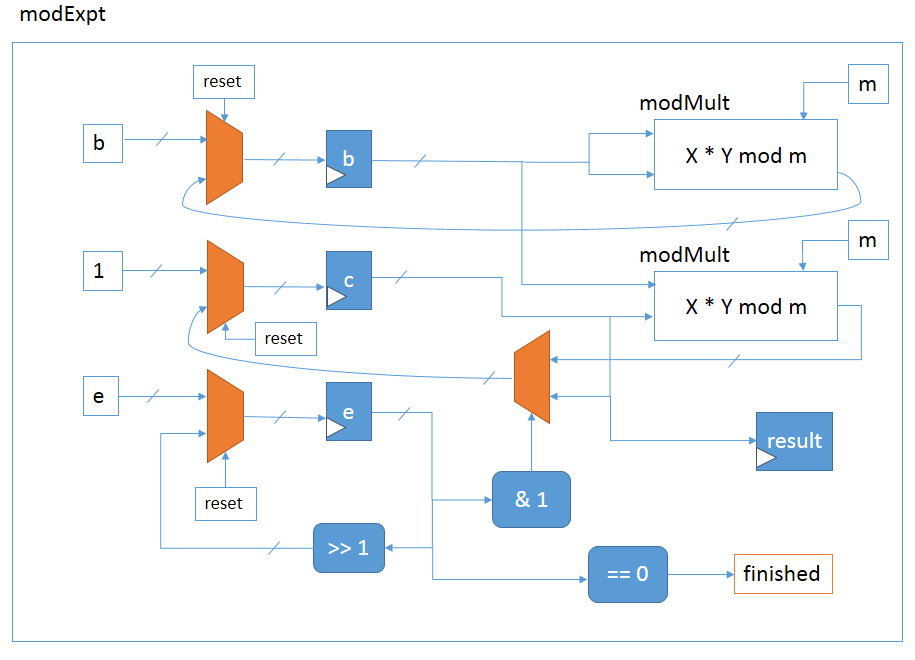
\includegraphics[width=\textwidth]{modexpt.png}
    \caption{Modular exponentiation}
    \label{fig-expt}
  \end{centering}
\end{figure}

\subsection{Interleaved Modular Multiplier}
The interleaved modular has the advantage of not requiring long multiplies, and works with
only left shifts, addition, subtraction, and comparison. Unfortunately, a step of the 
algorithm requires comparing the entire length of the data in the worst case. Additionally,
there are 3 possible add/subtract steps at every step of the algorithm. Therefore, the propagation delay
of each step of the algorithm may be prohibitive without pipelining. We will first investigate the
naive, unpipelined approach and see if it offers acceptable (100s of millisecond) performance. If it 
does not meet this target, then we will explicitly break the data into chunks to increase
the clock speed. 

An overview of the module is pictured in Figure \ref{fig-inter}.

\begin{figure}
  \begin{centering}
    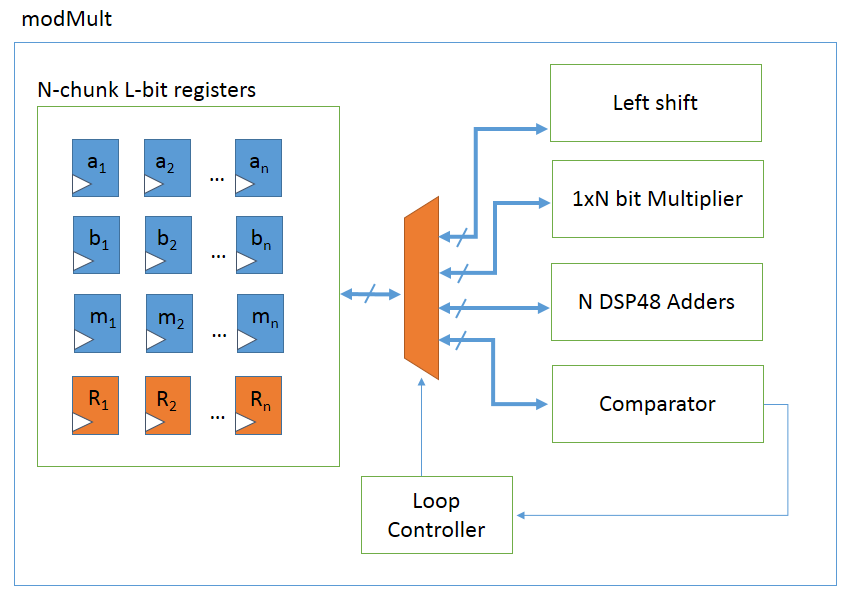
\includegraphics[width=\textwidth]{modmult.png}
    \caption{Interleaved modular multiplication}
    \label{fig-inter}
  \end{centering}
\end{figure}

\subsection{Naive Modular Multiplier}
An alternative to interleaved modular multiplication is the Naive approach.
The naive modular multiplier does not use any of the specialized algorithms
specifically tuned for hardware implementations.
This algorithms is unlikely to fit on the FPGA,
but might be interesting to implement as a point of comparison.
Particular bottlenecks of this implementation include the 2048 bit width result from the multiply block
resulting in a very long implementation for {\tt dbl\_modulus},
and the fact that such a multiplication is necessary at all.

An overview of this module is pictured in Figure \ref{fig-naive}.

\begin{figure}
  \begin{centering}
    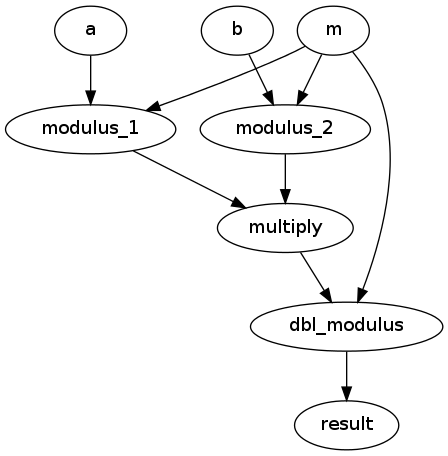
\includegraphics[width=0.4\textwidth]{modMultGraph.png}
    \caption{Naive modular multiplication}
    \label{fig-naive}
  \end{centering}
\end{figure}

\section{Implementation Status and Planned Exploration}
Since the main focus of our project is divided between the two important modules: modular exponentiator and modulus multiplier, we decided to pursue implementing these modules first.  At the beginning of this task, we had not decided upon integer representation; therefore, we were required to build multiple interfaces to test different types of data.  \\


\subsection{Implemented Modules}
The modules we implemented are:  {\tt SceMiLayer.bsv, RSAPipeline.bsv, RSA.bsv, RSAPipelinetypes.bsv,  ModMultIlvd.bsv, ModExpt.bsv, Memory.bsv}

\begin{description}
  \item[SceMiLayer.bsv] We developed two SceMiLayer modules to test different types of designs: one for importing vmh files, and another for importing libgcrypt for simulating our c code.  
  \item[RSAPipeline.bsv] This pipeline is based off the audio pipeline in the previous labs.  It's interfaces with SceMiLayer to retrieve input data and push output data to the test bench.
  \item[RSAPipelinetypes.bsv] This is the general header file where we define all constant values.  This will make the overall product modular and easy for others to change core elements of design such as number of bits per chunk.
  \item{RSA.bsv} This is a dedicated alternative driver for the RSA module that performs cosimulation with libgcrypt
  \item[ModMultIlvd.bsv] The interleaved modulus multiplier based on the Montgomery Algorithm.  This function computes $a*b$ mod $m$.
  \item[ModExpt.bsv] The modulus exponentiator described in section ?.  This module created two modulus multiplier to computer $b^e$ mod $m$.
  \item[Memory.bsv] This memory module implements BRAM functions: initialize, put, and get.  
\end{description}

The system is presently working correctly for 1024 bit RSA operations in simulation. The design performs software co-simulation using libgcrypt: the robust software library
 performs the same operations as the hardware RSA module, and compares the results at intermediate steps. It takes approximately 30 seconds to simulate one RSA operation, and
it is possible to perform randomized, long-term verification of the target module. 

\subsection{Integer Representation Explorations}
\begin{enumerate}
\item The first interface was a simple {\tt Int\#(1024)} representation. We created a simple adder in order to synthesize our design.
\item The second type of interface is most similar to our C implementation where integers are stored as 64 - 16 bit chunks.
\item The third type of interface uses BRAM to store chunks of the integer throughout the implementation. (This is currently incomplete)
\end{enumerate}
\subsubsection{Difficulties Encountered}
We created a simple adder in order to synthesize our design.  Since we had doubts about the success of this representation this was a vital step before continuing our design. Our concerns were well-founded for the simple {\tt Int\#(1024)} representation: the simple addition of two {\tt Int\#(1024)} were unable to synthesize.
\subsection{Planned Exploration}

\subsubsection{Trade-Offs: Cycle Time Estimation}

There are two major loops that run in the algorithm: the exponentiation loop,
and the modular multiplication loop. Each loop performs a bitwise operation
on the data, so it needs to perform a cycle for every bit of data. For a
1024 bit block size, both the outer (exponentiation) and inner (multiplication)
loops will require 1024 cycles. Therefore, at the minimum, the algorithm
requires ${N}^2$ cycles to perform one operation. However, since we were unable
to synthesize a 1024 bit wide adder, we will have to operate on the data
in chunks. This necessitates adding additional nested (pipelined) loops
inside the algorithm.

For a N-bit block size with M chunks, we would need to perform an additional $\frac{2N}{M}$
cycles of addition and $\frac{N}{M}$ cycles of comparison within every multiplication step in
the worst case. Therefore, the worst case cycle count is given by:

\begin{equation}
cycles_{worst}=\frac{3N^{3}}{M}
\end{equation}

For a 32-bit chunk size (N = 1024, M = 64), we would require 100 million cycles
to complete an operation on the block. However, this performance is very unlikely and
safe to ignore. 

The best case clock speed would require only a single comparison (detecting a difference
in the first chunk and aborting the full length) and no additional additions,
which would defined by

\begin{equation}
cycles_{best}=N\cdot (N+1)
\end{equation}

For a 32-bit chunk size, this would necessitate a clock speed of 5 MHz to meet the
performance of the Raspberry Pi.

The average case is similar in performance to the best case. In an empirical benchmark
using our cycle-accurate simulation, we calculated the following performance for 16-bit
chunk size:

\begin{equation}
cycles_{empirical}=1.6\cdot{N}^2
\end{equation}

Using this estimate, we will require a clock speed of 6 MHz to meet the Raspberry Pi performance, and
a clock speed of 60 MHz to meet the performance of a modern dual core processor. To improve performance further, 
it is possible to optimize the processing requirements on the required comparison step in the interleaved
modular multiply. It may be possible to explore faster comparison architectures by saving intermediate 
results from previous cycles.

\subsection{Design Exploration}
One of the major trade offs in our design is cycle period and number of cycles per encryption/decryption. 
During our preliminary synthesis exploration, we found that we cannot run the operation unpipelined on the FPGA:
the maximum frequency we can support mapped to the device is 25MHz.
In week 5, we will investigate timing violations and
modify our modules to operate on chunks of date (pipelining the design).  

While more detailed study of the synthesis reports will be needed to confirm this,
we believe that by far the greatest contributor to the critical path in the design are 1024 bit ripple-carry adders.
As such, in order to increase the clock frequency, we'll have to break these into sections.
These adders only occur in the modular multiplication module, and incidentally,
this module is where the vast majority of execution time is spent.
If an adder were broken into 4 chunks (for example) then it might take up to 13 or 14 (correspondingly shorter)
clock cycles to complete one iteration of the modular multiplier.

However, this suggests that a modular multiplier might be able to perform multiple computations in parallel.
It would be quite a bit of work to arrange,
but we might be able to have several computations cycling through the circular pipeline at once.
Each would have to be assigned a nonce in order to properly reorder results as they come out,
but there's no reason in principle that a single modular multiplier couldn't perform all the computations
for several independent modular exponentiators in parallel.
Naturally though, this goes somewhat beyond the original scope of the project,
and as we are all busy we hesitate to commit to taking on ever more complex tasks.

\section{Verification}
To verify the functionality of the RSA module, we initially separately 
compare the results of the encryption and decryption blocks to the results
of a software implementation. The two private keys for encryption and
decryption modules are passed by SceMi into the hardware. A SceMi testbench
pushes a message to the encryption block, along with an enable signal, message,
and public key of the software test-bench. The module generates an encrypted message,
and the software test-bench uses its private key to decrypt and verify the 
correctness of the encrypted message.

For decryption, the process is reversed: the test-bench passes in an 
encrypted message instead of plain-text, and the decryption module uses
the private key of the software test-bench to decrypt the message. The test-bench
verifies the plain-text for correctness.

After individual testing of the blocks, we will add support for confirming the signature
(authenticity checking) of the transmitted message. The test-bench will hash the plain-text
message before encryption, and use the private key as the exponent (as if it was decrypting
the hash). The hardware decryption module will use the test-bench's public key as the exponent
(as during encryption) to retrieve the hash as calculated by the sender. If the hash of the
decrypted message matches the original hash, then the message is genuine. The test-bench
will purposefully tamper with the encrypted message to prove the correctness of the 
signature detection mechanism. 

To prove correctness to the instructors, a simple test-bench will feed plain-text into an
encryption-decryption block pair (connected via a FIFO).


\end{document}  
